\chapter{Mathematical and graphical description of system}
\label{ap:systemOverview}
\graphicspath{{Appendix3/Appendix3Figures/},{Chapter1/Chapter1Figures/},{Chapter4/Chapter4Figures/}}

In this appendix a graphical and mathematical derivation for the system is given. It is shown through mathematical derivation how the pgmpy software can predict the student number and answer given the probability distributions and evidence. It should be noted that the software exploits additional methods in calculating these values in an efficient manner.

\section{High-level overview}

\begin{figure}
  \centering
  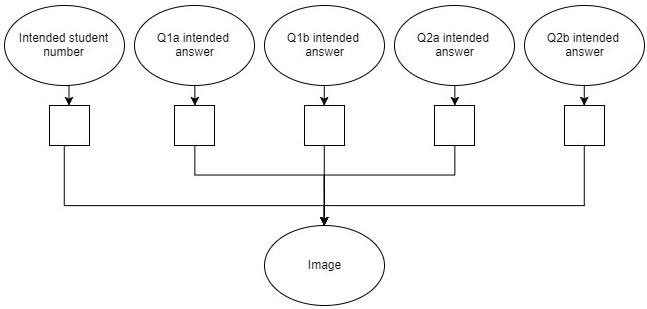
\includegraphics[width=11cm]{systemOverview}\\
  \caption{System overview.}
  \label{fig:appOverview}
\end{figure}
\nomenclature[S]{$A$}{Random variable representing an answer for a specific question}
\nomenclature[S]{$I$}{Random variable representing the test image}
\nomenclature[S]{$S$}{Random variable representing the possible student number}
As described in Chapter \ref{ch:Introduction}, the system can fundamentally be represented with 6 information nodes. These nodes are shown in Figure \ref{fig:appOverview}. The student has 5 pieces of information that he/she wants to portray, signifying the first 5 nodes. Those 5 nodes give rise to the image, representing the last node. At its core the system is tasked with inferring two types of conditional probabilities namely $P(S/I)$ and $P(A/I)$. The random variables $S$ and $A$ represent all the possible values that the student number and answers can possibly have. The image, $I$, is also a random variable representing the total number of possible states the image can take. Each image has a width and length of 1 240 by 1 754 pixels. For every pixel there are 256 possible values, ranging from 0.0 to 1.0. Thus the number of possible images are in the range of 1 240 $\times$ 1 754 $\times$ 256. To practically represent this, more detailed derivations and assumptions is needed. These derivations are described in the next sections. 
 
%The aim of the software is to maximize the likelihood of those probability distributions indicating the correct answers.
%The reason the problem is represented in a probabilistic way is due to the fact that different images are going to be generated every time a test is written. This is true even when the same information is going to be portrayed. Everytime a student writes a test he/she is going to write in different ways. A probabilistic graphical model (PGM) is thus used to describe this system and its inner operations. For a more detailed explanation on PGM's, refer to Section \ref{sec:PGM}.  The blocks in Figure \ref{fig:systemOverview} represent additional processing that is described in the following sections.

\section{The student answer}
In Section \ref{sec:studentAnswer}, it was determined that the student's answer can be calculated by combining the intended sign and digits of each column separately. This is attributed to the fact that these digits are independent of one another, as seen in Figure \ref{fig:appAns}. 

\begin{figure}
  \centering
  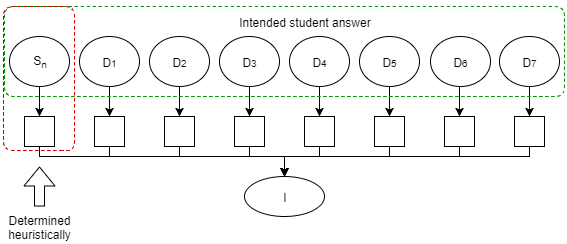
\includegraphics[width=10cm]{appAns}\\
  \caption{Graphical setup of determining student answer.}
  \label{fig:appAns}
\end{figure}
\nomenclature[S]{$Sn$}{Random variable representing the sign of a specific answer}
\nomenclature[S]{$D_i$}{Random variable representing a digit in column $i$ for a answer or student number block}
The intended digit in a certain column is not influenced by what the values in the other columns are. This independence property is thus described by\begin{align}
% \nonumber to remove numbering (before each equation)
  P(A/I) =  P(Si/I)P(D_1/I)...P(D_7/I),
\label{eqn:ansIndep}
\end{align}
where $A$ and $I$ again represent an answer  for a specific question and the image, respectively. The random variable $Si$ represents the sign of the answer.

To find the most probable answer, only $P(Sn/I)$ and $P(D_{1-7}/I)$ need to be calculated. Using image processing techniques described in Section \ref{ch:ImageProcessing}, $P(Si/I)$ can simply be determined heuristically by determining the probability of the bubble being coloured in, underneath the sign. Thus the only values yet to calculate is $P(D_{1-7}/I)$ and derived in the next section.

\section{The intended digit}

\begin{figure}
  \centering
  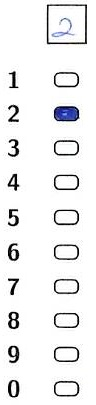
\includegraphics[width=1cm]{column}\\
  \caption{Column with evidence that gets considered for the calculation of an intended digit.}
  \label{fig:column}
\end{figure}

In determining an intended digit there are 11 information nodes to use as evidence. These nodes represent the 10 bubbles and character block, as shown in Figure \ref{fig:column}. Extra nodes are also added to symbolise the intended bubbles as described in Section \ref{sec:studentDigit}. The first bubble might sometimes incorrectly be associated with digit 0. Thus even if the student intended the digit 0 as an answer, the intended bubble of that student was actually the bubble for digit 1.

\begin{figure}
  \centering
  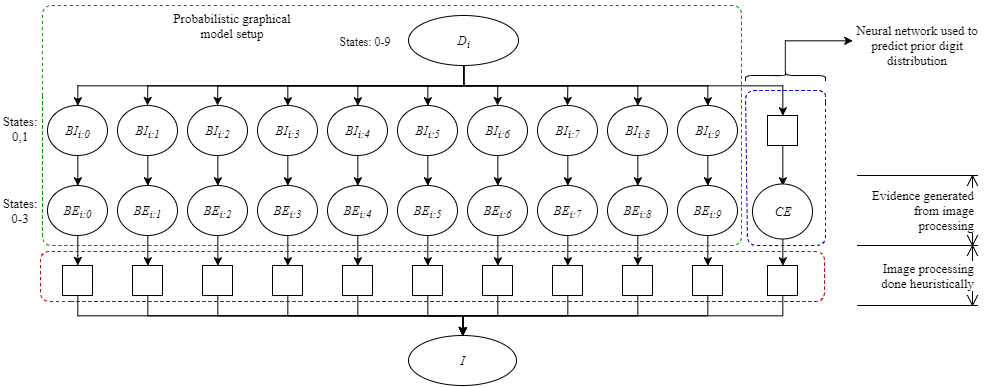
\includegraphics[width=16cm]{appDigit}\\
  \caption{Graphical setup of determining intended digit.}
  \label{fig:appDigit}
\end{figure}
\nomenclature[S]{$BE_i$}{Random variable representing bubble evidence obtained form image processing of the digit at index $i$}
\nomenclature[S]{$CE_i$}{Random variable representing a character evidence obtained form image processing at and arbitrary index $i$}

The probability of each column's digit is describe by $P(D_i/I)$. This value represents the probability of each of the 10 digits being written down in column $i$ . We know that the digit evidence is calculated heuristically using image processing. Each bubble thus has an evidence value with 4 possible states, namely not filled-in, crossed out, partially filled-in and completely filled-in. Thus the estimate of the intended digit is now represented by $P(D_i/I,BE_i,CE_i)$. $BE_i$ and $CE_i$ represents all the bubble and character evidence for that digit. As seen in Figure \ref{fig:appDigit}, $D_i$ and $I$ becomes independent from one another given the values of $BE_i$ and $CE_i$. Thus the probability of the intended digit is now given by $P(D_i/BE_i,CE_i)$.
\nomenclature[S]{$BI_i$}{Random variable representing the bubbles the student to colour in for digit $i$}
$BE_i$ is further described by 
\begin{align}
% \nonumber to remove numbering (before each equation)
  P(BE_i) =  P(BE_{i:0},BE_{i:1},...,BE_{i:9}),
\label{eqn:ansIndep}
\end{align}
where  $P(BE_{i:j})$ represents the digit i at bubble j. $BI_i$ is then represented by
\begin{align}
% \nonumber to remove numbering (before each equation)
  P(BI_i) =  P(BI_{i:0},BI_{i:1},...,BI_{i:9}),
\label{eqn:ansIndep}
\end{align}
where  $P(BI_{i:j})$ represents the digit i at bubble j.

$P(D_i/BE_i,CE_i)$ can now be represented by
\begin{align}
% \nonumber to remove numbering (before each equation)
  P(D_i/BE_i,CE_i)	=  \sum_{\forall BI_i}^{}  P(D_i,BI_i/BE_i,CE_i)\\
  					=  \sum_{\forall BI_i}^{}  \frac{P(BE_i,CE_i/D_i,BI_i)P(D_i,BI_i)}{P(BE_i,CE_i)}.
\label{eqn:ansEqn2}
\end{align}

In Equation \ref{eqn:ansEqn2}, the intended bubble term is brought in by making use of the sum rule. Bayes' rule is then applied. In Figure \ref{fig:appDigit}, $BE_i$ and $CE_i$ is seen to be independent when $D_i$ or $BI_i$ is known. Further it is observed that $BE_i$ is only reliant on $BI_i$ and $CE_i$ on $D_i$. Thus by applying an additional product rule it is determined that
\begin{align}
  P(D_i/BE_i,CE_i) =  \sum_{\forall BI_i}^{}\frac{P(BE_i/BI_i)P(BI_i/D_i)P(CE_i/D_i)P(D_i)}{P(BE_i,CE_i)}.
\label{eqn:ansEqn3}
\end{align}

Bayes' rule also provides us with,
\begin{align}
  P(CE_i/D_i)	=  \frac{P(D_i/CE_i)PCE_i)}{P(D_i)}.
\label{eqn:ansEqn4}
\end{align}

Now by factoring out all the constant terms out of the summation the equation reduces to,
\begin{align}
  P(D_i/BE_i,CE_i) =  \frac{P(CE_i)}{P(BE_i,CE,i)}\sum_{\forall BI_i}^{}P(BE_i/BI_i)P(BI_i/D_i)P(D_i/CE_i).
\label{eqn:ansEqn5}
\end{align}
The constant terms gets ignored in the pgmpy package due to them only being normalizing terms. Once the summation has been calculated the software simply normalizes the resulting values without needing those terms. Thus only $P(BE_i/BI_i)$, $P(BI_i/D_i)$ and $P(D_i/CE_i)$ are needed.

$P(BE_i/BI_i)$ and  $P(BI_i/D_i)$ are both terms that is deduced from training. The final term that is needed is $P(D_i/CE_i)$. This term is efficiently represented through the use of a neural network. Thus the PGM system can successfully infer the digit probabilities and thus the student answer with these 3 distributions specified. A derivation on the student number probability is discussed next.

\section{The student number}
\nomenclature[S]{$DE$}{Random variables representing a digit evidence obtained form image processing}
\nomenclature[S]{$DI$}{Random variables all the digit intended by the student}
As state in Section \ref{sec:studentNumber}, the assumption of independence between digits does not hold in the case of a student number. The reason for this is, because every 8 digit number is not equally likely to be a student number. Only student numbers that are valid needs to be considered as a possible state that the student number node can take. This node has approximately $900$ states, depending on the number of student numbers. The student number graph can be seen in Figure \ref{fig:stdNum}. 

A derivation for $P(S/I)$ is needed next. As stated previously, $S$ represents a random variable over all the possible student numbers. $I$ again represents the image. We know that the digit evidence is calculated heuristically using image processing. Thus the estimate of the student number is now represented as $P(S/I,DE)$. $DE$ now represents all the bubble and character evidence. As seen in Figure \ref{fig:stdNum}, $S$ and $I$ becomes independent from one another given the values of $DE$. Thus the probability of the intended digit is now given by $P(S/DE)$.

\begin{figure}
  \centering
  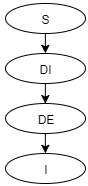
\includegraphics[width=2cm]{appStdNum}\\
  \caption{Graphical setup of determining student number.}
  \label{fig:stdNum}
\end{figure}

$DE$ is further described by 
\begin{align}
% \nonumber to remove numbering (before each equation)
  P(DE) =  P(BE_1,CE_1,BE_2,CE_2,...,BE_8,CE_8).
\label{eqn:ansIndep}
\end{align}

$DI$ is described by,

\begin{align}
% \nonumber to remove numbering (before each equation)
  P(DI) =  P(D_1,D_2,...,D_8).
\label{eqn:ansIndep2}
\end{align}

$P(S/DE)$ can now be represented by
\begin{align}
% \nonumber to remove numbering (before each equation)
  P(S/DE)	=  \sum_{\forall DI}^{}  P(S,DI/DE)\\
  					=  \sum_{\forall DI}^{}  \frac{P(BE/S,DI)P(S,DI)}{P(DE)}.
\label{eqn:stdEqn2}
\end{align}

In Equation \ref{eqn:stdEqn2}, the digit intended term, $DI$, is brought in by making use of the sum rule. Bayes' rule is then applied as shown.

In Figure \ref{fig:stdNum}, $DE$ is seen to be independent from $S$ if $DI$ is known and thus,

\begin{align}
% \nonumber to remove numbering (before each equation)
  P(S/DE)	=  \sum_{\forall DI}^{}  \frac{P(BE/DI)P(DI/S)P(S)}{P(DE)}.
\label{eqn:stdEqn3}
\end{align}

Finally from the digit and student number graph structure the following independence properties are also known,

\begin{align}
P(DE/ID) = P(BE_1/BI_1)P(CE/D_1)...P(BE_8/BI_8)P(CE/D_8)\\
\label{eqn:stdEqn4}
\end{align}

$P(S)$ can be initialized as an equal distribution, because every student number has the same likelihood in a given test. $P(DI/S)$ are values that are trained from data using the independence property, 
\begin{align}
P(DI/S) = P(D_1/S)...P(D_8/S).
\label{eqn:stdEqn4}
\end{align}
This value symbolizes the probability that the user intended to write down a digit given that student number. If the first digit of the student number is 1, the first intended digit will have a high probability of being 1. Thus these two random variables are strongly correlated. The only values that still need to be calculated are thus $P(DE/ID)$. Using the indepenency property of \begin{align}
P(DE/ID) = P(BE_1/BI_1)P(CE/D_1)...P(BE_8/BI_8)P(CE/D_8),
\label{eqn:stdEqn4}
\end{align}
the intended digit model's conditional distributions can be used. The two PGM models can now be fully defined and used to infer the intended student entries from an image.